\noindent


%%%%%%%%%%%%%%%%%%%%%%%%%%%%%%%%%%%%%%%%%%%%%%%%%%%%%%%%%%%%%%%%%%%%%%%%%%%%%%%%%%%%%%%%%%%%%%%%%%%%%%%%%%%%%%
%%%%%%%% WEAK AUTOMATA TO NDB %%%%%%%%%%%%%%%%%%%%%%%%%%%%%%%%%%%%%%%%%%%%%%%%%%%%%%%%%%%%%%%%%%%%%%%%%%%%%%%
%%%%%%%%%%%%%%%%%%%%%%%%%%%%%%%%%%%%%%%%%%%%%%%%%%%%%%%%%%%%%%%%%%%%%%%%%%%%%%%%%%%%%%%%%%%%%%%%%%%%%%%%%%%%%%


In this appendix we give a more detailed proof of Theorem \ref{thm:nmso_autofor}.

\begin{definition} Let $B = \{b_1,\dots,b_k\}$ and $P = \{p_1,\dots,p_j\}$ be two finite collection of set variables, representing respectively the states of an B\"{u}chi automaton and the propositional letters forming the labels of a $C$-labeled tree. In table \ref{fig:tableWFMSOFormulae} we fix some abbreviations for $\nmso$ formulae, expressing concepts which are easily seen to be definable in this logic. All valuations (for which we use the notation $\|\cdot\|$) are referred to a fixed tree $\model$. Observe that for each $p_i \in P$ the set $\|p_i\|$ is determined by the labelling function $\V:T\rightarrow C$ of $\model$.

\begin{table}[ht]\centering
%\begin{center}
\begin{tabular}{|p{1.8cm}|p{11.5cm}|}
\hline
\textbf{Formula} & \textbf{Meaning} \\ \hline \hline
$\mathit{Pfix}_z(p)$ & The set $\|p\|$ is a prefix of the subtree $\model.{\|z\|}$. \\
\hline
$\mathit{Root}(x)$ & The node $\|x\|$ is the root of $\model$. \\
\hline
$\mathit{Front}(p)$ & The set $\|p\|$ is a frontier of $\model$. \\
\hline
$\mathit{State}_{a,B}(x)$ & $a$ is the only set variable in $B$ such that the node $\|x\|$ is in $\|a\|$ (we say that \emph{the state $a$ marks $\|x\|$}). \\
 \hline
$\mathit{Part}_B(p)$ & Each node in the set $\|p\|$ is marked with a unique $a \in B$. \\
\hline
$\mathit{Trans}_{B,C}(p)$ & For each node $\|x\| \in \|p\|$, state $a \in B$, label $c\in C$, if $a$ marks $\|x\|$ and $\|x\|$ is labeled with $c$ then $\tmap(a,c)$ holds in $\R{\|x\|}$ (this latter condition is rendered by relativizing all quantifiers of $\tmap(a,c)$ to elements of $\R{\|x\|}$). \\
\hline
\end{tabular}
%\end{center}
\label{fig:tableWFMSOFormulae}\caption{{Abbreviations for $\nmso$ formulae}}\end{table}

We also define $\mathit{Surv}_{B,C}(p)$ as $\mathit{Part}_B(p) \wedge \mathit{Trans}_{B,C}(p)$, where $\mathit{Part}_B(p)$ and $\mathit{Trans}_{B,C}(p)$ are given as in table \ref{fig:tableWFMSOFormulae}. Intuitively, if $\mathit{Surv}_{B,C}(p)$ holds then player $\exists$ is guaranteed to have a legitimate move available from any node $\|x\|$ in $\|p\|$, assigning exactly one state to each $t \in \R{\|x\|}$.
\end{definition}


\begin{definition}\label{DEF_K_m} Let $\baut$ and $\overline{\baut}$ be B\"{u}chi automata, with $B = \{b_1,\dots,b_k\}$ and $F\subseteq B$ respectively the set of states and of accepting states of $\baut$. For each $b \in B$, we define by induction a sequence of formulae $K_i^b(x)$. Put $K_0^{b}(x) := \top$. The formula $K_{i+1}^{b}(x)$ is given as follows:

\begin{align*}
% \nonumber to remove numbering (before each equation)
  K_{i+1}^{b}(x)\ :=\ & \forall p\ \exists p^{\prime}\ \exists b_1\dots\exists b_k\ \Bigg(\mathit{Pfix}_x(p) \rightarrow
                       \bigg(p \subseteq p^{\prime} \wedge \mathit{Pfix}_x(p^{\prime}) \wedge \mathit{Surv}_{B,C}(p^{\prime}) \wedge
                       \mathit{State}_{b,B}(x)  \\
                       & \wedge \Big(\forall y\ \big(y\in \mathit{Front}(p^{\prime})\rightarrow 
                       (\bigvee_{b^{\prime} \in F} (\mathit{State}_{b^{\prime},B}(y) \wedge K_i^{b^{\prime}}(y)))\big)\Big)\bigg)\Bigg).
\end{align*}
Let $m$ be the product of the cardinalities of the carriers of $\baut$ and $\overline{\baut}$. The formula $\varphi_{\baut,\overline{\baut}} \in \nmso$ is defined by putting
\begin{equation*}
    \varphi_{\baut,\overline{\baut}}\ :=\ \exists y\ (\mathit{Root}(y) \wedge K_{m+1}^{b_I}(y)).
\end{equation*}
\end{definition}

Observe that, for any $k < \omega$, $K_k^b(x)$ is a formula of $\nmso$. We refer to section \ref{sec:weakgoeswell} for an intuitive reading of the semantics of $K_{i+1}^{b}(x)$.

Our next goal is to show the main result of section \ref{sec:weakgoeswell}.

\begin{trivlist}
\item \textbf{Theorem~\ref{thm:nmso_autofor}}. \ThWeakAutToWFMSO
\end{trivlist}

In this aim, we fix the following terminology concerning a winning strategy $f$ for $\exists$ in some acceptance game $\mc{G}$: a basic position $(a,s)$ is \emph{$f$-admissible} if there is some $f$-conform match of $\mc{G}$ where $(a,s)$ occurs. %Recall that functional strategies are the ones assigning \emph{exactly one state} to each successor of the node under consideration. Then we can observe that, if $f$ is functional, each node $s$ of $\model$ can be associated with a unique state $a_s$ of $\aut$ and a unique $f$-admissible position $(a_s,s)$.

In the next we fill in the details of the proof sketch provided in section \ref{sec:weakgoeswell}. As stated there, we can assume to work with B\"{u}chi automata $\baut$ and $\overline{\baut}$, equivalent respectively to $\aut$ and the weak $\MSO$-automaton $\overline{\aut}$ recognizing the complement $\overline{\mathcal{L}(\aut)}$ of the tree language $\mathcal{L}(\aut)$. Then theorem \ref{thm:nmso_autofor} is an immediate consequence of the following proposition.

\begin{proposition} Let $\baut= \langle B,b_I,\tmap,F\rangle$ and $\overline{\baut} = \langle \overline{B},\overline{b}_I,\overline{\tmap},\overline{F}\rangle$ be B\"{u}chi automata such that $\mathcal{L}(\overline{\baut}) = \overline{\mathcal{L}(\baut)}$. Let $\varphi_{\baut,\overline{\baut}} \in \nmso$ be given in terms of $\baut$ and $\overline{\baut}$ according to definition \ref{DEF_K_m}. Over tree languages, we have that $\mathcal{L}(  \baut) = \|\varphi_{\baut,\overline{\baut}}\|$. \end{proposition}
%%%%%%%%%%%%%%%%%%%%%%%%%%%%%%%%%%%%%%%%%%%%%%%%%%%%%%%%%%%%%%%%%%%%%%%%%%%%%%%%%%%%%%%%%%%%%%%%%%%%%%%%%%%%%%%%%%%%%%%%%%%%%%%%%%%%%%%%%%%%%%%%%%%%%%%%%%%%%%%%%%%%%%%%
%%%%%%%%%%%%%%%%%%%%%%%%%%%%%%%%%%%%%%%%%%%%%%%%%%%%%%%%%%%%%%%%%%%%%%%%%%%%%%%%%%%%%%%%%%%%%%%%%%%%%%%%%%%%%%%%%%%%%%%%%%%%%%%%%%%%%%%%%%%%%%%%%%%%%%%%%%%%%%%%%%%%%%%%
%%%%%%%%%% PROOF TO BE REFINED ? %%%%%%%%%%%%%%%%%%%%%%%%%%%%%%%%%%%%%%%%%%%%%%%%%%%%%%%%%%%%%%%%%%%%%%%%%%%%%%%%%%%%%%%%%%%%%%%%%%%%%%%%%%%%%%%%%%%%%%%%%%%%%%%%%%%%%%%%%%%%%%%
%%%%%%%%%%%%%%%%%%%%%%%%%%%%%%%%%%%%%%%%%%%%%%%%%%%%%%%%%%%%%%%%%%%%%%%%%%%%%%%%%%%%%%%%%%%%%%%%%%%%%%%%%%%%%%%%%%%%%%%%%%%%%%%%%%%%%%%%%%%%%%%%%%%%%%%%%%%%%%%%%%%%%%%%
%%%%%%%%%%%%%%%%%%%%%%%%%%%%%%%%%%%%%%%%%%%%%%%%%%%%%%%%%%%%%%%%%%%%%%%%%%%%%%%%%%%%%%%%%%%%%%%%%%%%%%%%%%%%%%%%%%%%%%%%%%%%%%%%%%%%%%%%%%%%%%%%%%%%%%%%%%%%%%%%%%%%%%%%
\begin{proof} \begin{Iff-RL} Let $\model$ be a tree and $f$ be a winning strategy for $\exists$ in $\mc{G} = \agame(\baut,\mathbb{T})@(b_I,s_I)$, which we can assume to be functional by Remark \ref{rmk:Buchifunctional}. Since $f$ is winning then we are provided with an $\omega$-accepting sequence $(E_i)_{i < \omega}$ for $f$ over $\baut$ and $\model$, according to proposition \ref{PROP_Buchi_finite_segments}. Our goal is to show that $\mathbb{T} \models \varphi_{\baut,\overline{\baut}}$. In fact, it suffices to show the following statement.

\smallskip

\begin{claim}\label{CLAIM_WeakParityInWFMSO2} For each $i < \omega$, for each $(b,s)\in B\times T$, if $(b,s)$ is a winning position for $\exists$ in $\mc{G}$, then $\mathbb{T} \models K_i^{b}(x)$, with $\|x\| = s$. \end{claim}

\begin{proof}[Proof of Claim \ref{CLAIM_WeakParityInWFMSO2}]
We proceed by induction on $i$. Since $K_0^{b}(x) = \top$, the base case is trivial. Inductively, let $(b,s)$ be a winning position for $\exists$ in $\mc{G}$. We put $\|x\| = s$ and we claim that $\mathbb{T} \models K_{i+1}^{b}(x)$. Following the syntactic shape of $K_{i+1}^{b}(x)$, we let $\|p\|$ be an arbitrary prefix $E$ of $\mathbb{T}.s$. By definition of the sequence $(E_i)_{i < \omega}$, for each $i < \omega$ we have that $\mathit{Ft}(E_i) < \mathit{Ft}(E_{i+1})$, implying that there is some prefix $E_n$ in the sequence such that $E \subseteq E_n$. We pick $E_n \cap {T.s}$ as the witness for the set-variable $p^{\prime}$ in $K_{i+1}^{b}(x)$.

We still need to provide witnesses for set-variables $b_1,\dots,b_k$ occurring in $K_{i+1}^{b}(x)$. The idea is to let them be suggested by the strategy $f$. Since $f$ is functional, any node $s \in \model$ is associated with a unique $b_s \in B$ and a unique $f$-admissible basic position $(b_s,s)$. For each $b_j$ in $\{b_1,\dots,b_k\}$, we define its valuation by putting
\begin{eqnarray}\label{EQ_b_j_eval}
% \nonumber to remove numbering (before each equation)
  \|b_j\| &:=& \{s \in (E_n \cap T.s)\ |\ b_j = b_s\}.
\end{eqnarray}
Since $E_n \cap T.s$ is well-founded then $\|b_j\|$ is noetherian, so that it is a legitimate witness for $b_j$ according to the semantics of $\nmso$.

The subformula ${Surv}_{B,C}(p^{\prime})$ of $K_{i+1}^{b}(x)$ holds because the strategy $f$ is assumed to be functional and winning for $\exists$, so in particular it is functional and surviving for $\exists$ in $E_n \cap T.s = \|p^{\prime}\|$. Concerning the subformula $\mathit{State}_{b,B}(x)$, by assumption $(b,s)$ is a winning position for $\exists$. This means that $b$ is the unique set-variable marking $s = \|x\|$ according to \eqref{EQ_b_j_eval}, so that $\mathit{State}_{b,B}(x)$ holds. It remains to show the statement
\begin{eqnarray}\label{EQ_forallinF_K_m}
% \nonumber to remove numbering (before each equation)
  \forall y\ (y\in \mathit{Front}(p^{\prime})\rightarrow (\bigvee_{b \in F} \mathit{State}_{b,B}(y) \wedge K_i^{b}(y))).
\end{eqnarray}
For this purpose, let $\|y\|$ be some node on the frontier of $E_n = \|p^{\prime}\|$. By \eqref{EQ_b_j_eval} and the fact that $f$ is functional, there is a unique set-variable $\|b\|$ marking $\|y\|$, such that $(b,\|y\|)$ is $f$-admissible. Therefore $(b,\|y\|)$ is a winning position for $\exists$ in $\mc{G}$, and $K_i^{b}(y)$ holds by inductive hypothesis. The fact that $b$ is in $F$ follows from properties of the frontier of $E_n$ as in definition \ref{DEF_accepting_sequence}.
\end{proof}

By applying claim \ref{CLAIM_WeakParityInWFMSO2} to the winning position $(b_I,s_I)$ we have that $\mathbb{T} \models K_{n}^{b_I}(x)$ for each $n<\omega$, with $x$ witnessed by $s_I$. Then in particular $\mathbb{T} \models \exists x\ (\mathit{Root}(x) \wedge K_{m+1}^{b_I}(x))$. This completes the proof of direction $(\Rightarrow)$.

\end{Iff-RL}
\begin{Iff-LR} Let $\model$ be a tree where $\varphi_{\baut,\overline{\baut}}$ is true. We need to show that $\model$ is accepted by $\baut$.

The idea of the proof is as follows. Suppose by way of contradiction that $\baut$ does not accept $\mathbb{T}$. Then the tree $\model$ is accepted by $\overline{\baut}$. Let $\overline{f}$ be a functional winning strategy for $\exists$ in $\agame(\overline{\baut},\mathbb{T})$. Suppose that we can prove from the previous assumptions the existence of an $m$-trap for $\baut$ and $\overline{\baut}$. Then by proposition \ref{PROP_Rabin_trap} we have that $L(\baut) \cap L(\overline{\baut}) \neq \emptyset$, contradicting the fact that $L(\overline{\baut}) = \overline{L(\baut)}$.

In order to complete the proof of direction $(\Leftarrow)$, it remains to verify the following claim.

\smallskip

\begin{claim}\label{CLAIM_WeakParityInWFMSO3} There exists an $m$-trap for $\baut$ and $\overline{\baut}$.\end{claim}

\begin{proof}[Proof of Claim \ref{CLAIM_WeakParityInWFMSO3}] By definition \ref{DEF_Rabin_trap}, we have to to provide the following components:
\begin{enumerate}
  \item a strictly increasing sequence $(E_i)_{i\leq m}$ of prefixes of $\mathbb{T}$, with $E_0 = \{s_I\}$;
  \item a strategy $f^{B}$ for $\exists$ in $\mc{G}=\mc{A}(\baut,\mathbb{T})@(b_I,s_I)$ which is surviving for $\exists$ in $E_m$;
  \item a strategy $f^{\overline{B}}$ for $\exists$ in $\overline{\mc{G}}=\mc{A}(\overline{\baut},\mathbb{T})@(\overline{b}_I,s_I)$ which is surviving for $\exists$ in $E_m$;
  \item an $m$-accepting sequence $(G_i^{B})_{i\leq m}$ for $f^{B}$ over $\baut$ and $\mathbb{T}$;
  \item an $m$-accepting sequence $(G_i^{\overline{B}})_{i\leq m}$ for $f^{\overline{B}}$ over $\overline{\baut}$ and $\mathbb{T}$.
\end{enumerate}
Moreover, $(E_i)_{i\leq m}$, $(G_i^{B})_{i\leq m}$ and $(G_i^{\overline{B}})_{i\leq m}$ have to present the interleaving behavior described in definition \ref{DEF_Rabin_trap}.

\smallskip

We put the strategy $\overline{f}$ as witness for $f^{\overline{B}}$. By assumption $\overline{f}$ is a winning strategy for $\exists$ in $\overline{\mc{G}}$. Then, by proposition \ref{PROP_Buchi_finite_segments}, we are also given with an $\omega$-accepting sequence $(E^{\overline{f}}_i)_{i< \omega}$ for $\overline{f}$ over $\overline{\baut}$ and $\model$.

It remains to define the other components of the $m$-trap, which is what we do next. The idea is to define the surviving strategy $f^{B}$, the sequences $(E_i)_{i\leq m}$ and $(G_i^{B})_{i\leq m}$ by using the assumption that $\mathbb{T} \models \varphi_{\baut,\overline{\baut}}$. The last component, namely the sequence $(G_i^{\overline{B}})_{i\leq m}$, will be defined from $(E^{\overline{f}}_i)_{i< \omega}$.

\smallskip

The construction of the strategy $f^{B}$ and the sequences $(E_i)_{i\leq m}$, $(G_i^{B})_{i\leq m}$ and $(G_i^{\overline{B}})_{i\leq m}$ proceeds in stages, by induction on $i \leq m$. In particular, $f^{B}$ will be defined as the last element $f^{B}_m$ in a sequence of strategies $(f^{B}_i)_{i\leq m}$.

Given $i\leq m$, the inductive hypothesis that we want to maintain along the construction can be expressed as follows.

\bigskip
\begin{center}
\fbox{\parbox{13.4cm}{
\begin{enumerate}
  \item If $i < m$ then $\mathit{Ft}(E_{i}) \leq \mathit{Ft}(G_{i}^{B}) < \mathit{Ft}(E_{i+1})$, otherwise $i = m$ and $\mathit{Ft}(E_{i}) \leq \mathit{Ft}(G_{i}^{B})$.
  \item If $i < m$ then $\mathit{Ft}(E_i) \leq \mathit{Ft}(G_{i}^{\overline{B}}) < \mathit{Ft}(E_{i+1})$, otherwise $i = m$ and $\mathit{Ft}(E_{i}) \leq \mathit{Ft}(G_{i}^{\overline{B}})$.
  \item The sets $E_{i}$, $G_{i}^{B}$ $G_i^{\overline{B}}$ are prefixes of $\model$.
  \item The function $f^{B}_{i}$ is a strategy $\exists$ in $\mc{G}$ which is functional and surviving in $G^{B}_{i}$. If $i \geq 1$, then $f^{B}_{i}$ extends $f^{B}_{i-1}$.
  \item For each $s \in \mathit{Ft}(G^{\overline{B}}_i)$, there is a unique $\overline{b}_s \in \overline{B}$ such that the position $(\overline{b}_s,s)$ is $\overline{f}$-admissible; also, $\overline{b}_s$ is in $\overline{F}$.
  \item For each $s \in \mathit{Ft}(G^{B}_i)$, there is a unique $b_s \in B$ such that the formula $K_{m-i}^{b_s}(x)$ holds for $s = \|x\|$. The position $(b_s,s)$ is $f^{B}_i$-admissible; also, $b_s$ is in $F$.
\end{enumerate}
}}\hspace*{0.2cm}($\ddag$)
\end{center}

\bigskip

Let us first show why the different components form an $m$-trap if condition ($\ddag$) can be maintained. By ($\ddag . 4$) the strategy $f^{B} = f^{B}_m$ for $\exists$ in $\mc{G}$ would be functional and surviving in $G^{B}_{m}$. By ($\ddag . 1$) we have that $\mathit{Ft}(E_{m}) \leq \mathit{Ft}(G_{m}^{B})$, meaning that $f^{B}$ is also surviving in $E_{m}$, as requested by point 1 of the definition of $m$-trap (definition \ref{DEF_Rabin_trap}). For $f^{\overline{B}} = \overline{f}$, we know by assumption that $\overline{f}$ is functional and winning for $\exists$ in $\overline{\mc{G}}$. Since $E_m$ is a subset of $T$, then $f^{\overline{B}}$ is also surviving in $E_m$, as requested by point 2 of definition \ref{DEF_Rabin_trap}.

For points 3 and 4 of definition \ref{DEF_Rabin_trap}, we have to check that $(G_i^{B})_{i\leq m}$ and $(G_i^{\overline{B}})_{i\leq m}$ are $m$-accepting sequences respectively for $f^{B}$ and $f^{\overline{B}}$. For this purpose, there are three conditions to check according to the definition of accepting sequence (definition \ref{DEF_accepting_sequence}). The first condition is that $(G_i^{B})_{i\leq m}$ and $(G_i^{\overline{B}})_{i\leq m}$ are sequences of prefixes, which is given by ($\ddag . 3$). The second condition, on the relation between frontiers of each $G_i^{B}$, $G_i^{\overline{B}}$ and $E_i$, is given by ($\ddag . 1$) and ($\ddag . 2$). Concerning the third condition of definition \ref{DEF_accepting_sequence}, for each $i\leq m$, the requirements on $\mathit{Ft}(G_i^{B})$ and $\mathit{Ft}(G_i^{\overline{B}})$ are fulfilled by ($\ddag . 5$) and ($\ddag . 6$).

The last two points of definition \ref{DEF_Rabin_trap}, concerning the interleaving of the frontiers of $(E_i)_{i\leq m}$, $(G_i^{B})_{i\leq m}$ and $(G_i^{\overline{B}})_{i\leq m}$, just correspond to ($\ddag . 1$) and ($\ddag . 2$). Therefore what we obtain is indeed an $m$-trap, provided that we are able to maintain condition ($\ddag$).

\bigskip

Now we proceed with the inductive construction. For the base case, let $E_0 := \{s_I\}$. We define the first element $G_0^{\overline{B}}$ in the sequence $(G_i^{\overline{B}})_{i\leq m}$ as the smallest prefix in the sequence $(E^{\overline{f}}_i)_{i< \omega}$ such that $E_0 \subseteq G_0^{\overline{B}}$, that is simply $E^{\overline{f}}_0$ because $(E^{\overline{f}}_i)_{i< \omega}$ is monotone.

In order to define $G_0^B$, we observe that the unique witness for $x$ in $\exists x\ (\mathit{Root}(x)\wedge K_{m+1}^{b_I}(x))$ must be $s_I$. Then, by putting $E_0$ as the witness of the variable $p$ in $K_{m+1}^{b_I}(x)$, we are provided with a prefix $G^{B}_0$ witnessing the variable $p^{\prime}$ in $K_{m+1}^{b_I}(x)$. We let such $G^{B}_0$ be the first element in the sequence $(G_i^{B})_{i\leq m}$.

In order to define the first surviving strategy $f^{B}_0$ in the sequence $(f^{B}_i)_{i\leq m}$, we fix valuations $\|p\|=E_0$ and $\|p^{\prime}\| = G^{B}_0$ in the formula $K_m^{b_I}(x)$ and we consider the witnesses for set-variables $b_1,\dots,b_k$ in $K_{m+1}^{b_I}(x)$. By definition of $K_{m+1}^{b_I}(x)$, for each node $s$ in $G^{B}_0$ there is a unique $b_s \in \{b_1,\dots,b_k\}$ such that $s \in \|b_s\|$. This yields a strategy $f^{B}_0$ for $\exists$ in $\mc{G}$ (actually, for partial matches which are played along nodes of $G^{B}_0$), which we define as follows:
 \begin{enumerate}
   \item $f^{B}_0$ is defined at the basic position $(b_I,s_I)$;
   \item given a basic position $(b_s,s) \in B \times G^{B}_0$ with $s \not\in \mathit{Ft}(G^{B}_0)$, we let $f^{B}_0$ suggest to $\exists$ a marking assigning $b_t$ to $t$, for each $t \in \R{s}$;
   \item we leave $f^{B}_0$ undefined on all other basic positions from $B \times T$.
 \end{enumerate}

Given prefixes $G_0^{\overline{B}}$ and $G_0^B$ as above, we define $E_1$ to be the smallest prefix of $\model$ such that $\mathit{Ft}(G_0^B) < \mathit{Ft}(E_1)$ and $\mathit{Ft}(G_0^{\overline{B}}) < \mathit{Ft}(E_1)$.

\smallskip

It remains to check that conditions $1-5$ in $(\ddag)$ hold for the base case. Condition $(\ddag .1)$, $(\ddag .2)$ and $(\ddag .3)$ are clear by construction of $E_0$, $G_0^{\overline{B}}$, $G_0^B$ and $E_1$. For condition $(\ddag .4)$, by assumption we have that $\mathit{State}_{b_I,B}(y)$ and $\mathit{Surv}_{B,P}(p^{\prime})$ hold, being subformulae of $K_m^{b_I}(x)$, with $\|p^{\prime}\| = G^{B}_0$ and $\|y\| = s_I$. By construction of the strategy $f^{B}_0$, this means that $f^{B}_0$ is functional and surviving for $\exists$ in $G^{B}_0$. Analogously, $(\ddag .5)$ holds because the subformula of $K_m^{b_I}(x)$ given as in \eqref{EQ_forallinF_K_m} is true, meaning that every node on the frontier of $G^{B}_0$ is associated with a unique accepting state of $\baut$ according to $f^{B}_0$. In order to fulfill condition $(\ddag .6)$, we observe that, by definition of $K_{m+1}^{b_I}(x)$, every node $s \in \mathit{Ft}(G^{B}_0)$ is associated with a basic position $(b_s,s) \in B \times T$, such that $b_s \in F$ and $K_{m}^{b_s}(x)$ holds for $s = \|x\|$.


\bigskip

Inductively, we consider the stage $j+1 \leq m$ of the construction. By inductive hypothesis, we are given with sequences $(E_i)_{i\leq {j+1}}$, $(G_i^{B})_{i\leq j}$, $(G_i^{\overline{B}})_{i\leq j}$ and a strategy $f^{B}_j$ for $\exists$ as in $(\ddag)$.

Analogously to the base case, we define $G_{j+1}^{\overline{B}}$ as smallest prefix in the sequence $(E^{\overline{f}}_i)_{i< \omega}$ which contains $E_{j+1}$. For the definition of $G_{j+1}^{B}$ and $f^{B}_{j+1}$, the key observation is that, by inductive hypothesis, for each node $s \in \mathit{Ft}(G^{B}_j)$ we can make the following assumptions:
 \begin{enumerate}
   \item the formula $K_{m-j}^{b_s}(x)$ holds, with $s = \|x\|$;
   \item the position $(b_s,s)$ is $f^{B}_j$-admissible.
 \end{enumerate}

We let $T.s \cap E_{j+1}$ be the witness for the set-variable $p$ occurring in $K_{m-j}^{b_s}(x)$. Then by definition of $K_{m-j}^{b_s}(x)$ we are provided with a prefix $G_{j+1}^{B,s}$ of $\model.s$ witnessing the variable $p^{\prime}$, such that ${T.s} \cap E_{j+1} \subseteq G_{j+1}^{B,s}$. Also we are provided with noetherian sets of nodes witnessing variables $b_1,\dots,b_k$. Analogously to the base case, this yields a strategy $f^{B,s}_{j+1}$ for $\exists$ in $\mc{G}$, which is defined as follows:
 \begin{enumerate}
   \item $f^{B}_{j+1}$ is defined at the basic position $(b_s,s)$;
   \item for each basic position $(b_t,t)\in B \times G_{j+1}^{B,s}$ with $t \not\in \mathit{Ft}(G_{j+1}^{B,s})$, we let $f^{B}_{j+1}$ suggest to $\exists$ a marking assigning $b_r$ to $r$, for each $r \in \R{t}$.
   \item we leave $f^{B}_{j+1}$ undefined on all other basic positions from $B \times T$.
 \end{enumerate}
In other words, $f^{B,s}_{j+1}$ is a strategy for $\exists$ in partial matches of $\mc{A}(\aut,\model)@(b_s,s)$, which is functional, surviving in $G_{j+1}^{B,s}$ and marks each node $t \in \mathit{Ft}(G_{j+1}^{B,s})$ with a unique state from $F$.

\smallskip

We define $G_{j+1}^{B} := G_{j}^{B} \cup \bigcup_{s \in \mathit{Ft}(G^{B}_j)} G_{j+1}^{B,s}$. Since $G_{j}^{B}$ is a prefix of $\model$ and for each $s \in \mathit{Ft}(G^{B}_j)$ the set $G_{j+1}^{B,s}$ is a prefix of $\model.s$, we have that $G_{j+1}^{B}$ is a prefix of $\model$. Next, we define $f_{j+1}^{B} := f_j^{B} \cup \bigcup_{s \in \mathit{Ft}(G^{B}_j)} f_{j+1}^{B,s}$, where the union of strategies just means the union of their graphs. In order to check that $f_{j+1}^{B}$ is indeed a function, observe that by inductive hypothesis $f_j^{B}$ is defined on basic positions in $B \times (G_{j}^{B} \setminus \mathit{Ft}(G_{j}^{B}))$. By construction, for each $s \in \mathit{Ft}(G^{B}_j)$, the strategy $f_{j+1}^{B,s}$ is defined on the union of $\{(b_s,s)\}$ and $B \times (G_{j+1}^{B,s} \setminus (G_{j}^{B} \cup \mathit{Ft}(G_{j+1}^{B,s})))$. Since $(b_s,s) \in \mathit{Ft}(G_{j}^{B})$, then the domains of $f_j^{B}$ and each $f_{j+1}^{B,s}$ are all disjoints. Therefore $f_{j+1}^{B}$ is uniquely defined on each basic position in its domain.

\begin{figure}[h]
  % Requires \usepackage{graphicx}
  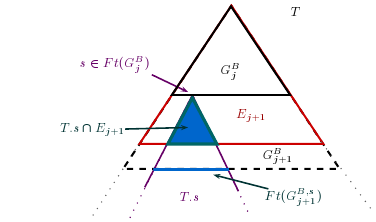
\includegraphics[width=8cm]{appendix/FIG_PropBuchiToWFMSO.png}\\
  \caption{\rm Construction of $G_{j+1}^B$}\label{FIG_PropBuchiToWFMSO}
\end{figure}

%For each $s \in \mathit{Ft}(G^{B}_i)$, the well-founded subtree $G_{i+1}^{B,s}$ and the strategy $f^{B,s}_{i+1}$ are defined as above.

%We briefly check that $G_{i+1}^{B}$ and $f_{i+1}^{B}$ have the desired properties. By construction for each $s \in \mathit{Ft}(G^{B}_i)$ we know that $\model_s \cap E_i\subseteq G_{i+1}^{B,s}$. It follows that $\mathit{Ft}(\model_s \cap E_i) \leq \mathit{Ft}(G_{i+1}^{B,s})$. By inductive hypothesis we also know that $\mathit{Ft}(G^{B}_i) < \mathit{Ft}(E_{i+1})$. Then it follows that \begin{equation}\label{EQ_frontiers_inductive_case}   \mathit{Ft}(E_i) \leq \mb{Ft}(\bigcup_{s \in \mathit{Ft}(G^{B}_i)} G_{i+1}^{B,s}) = \mb{Ft}(G_{i+1}^{B} \end{equation}


%The fact that $f_{i+1}^{B}$ is full, functional and surviving for $\exists$ in $\mc{A}(\baut,E_{i+1}^{B})@(b_I,s_I)$ can be checked as follows. By inductive hypothesis $f_{i}^{B}$ is full, functional and surviving for $\exists$ in $\mc{A}(\baut,E_{i}^{B})@(b_I,s_I)$.


Given $G_{j+1}^{\overline{B}}$ and $G_{j+1}^B$ as above, if $j+1 < m$ then we define $E_{j+2}$ to be the smallest prefix of $\model$ such that $\mathit{Ft}(G_{j+1}^B) < \mathit{Ft}(E_{j+2})$ and $\mathit{Ft}(G_{j+1}^{\overline{B}}) < \mathit{Ft}(E_{j+2})$. The check that all conditions in $(\ddag)$ hold for $G_{j+1}^{B}$, $f_{j+1}^{B}$ and $E_{j+2}^{B}$ is completely analogous to the base case.

We have just defined a strategy $f^{B}$, sequences $(E_i)_{i\leq m}$, $(G_i^{B})_{i\leq m}$ and $(G_i^{\overline{B}})_{i\leq m}$, such that for each $i \leq m$ condition $(\ddag)$ is respected. It follows that $\overline{f}$ and $f^{B}$ witness a trap for $\baut$ and $\overline{B}$ according to definition \ref{DEF_Rabin_trap}. This concludes the proof of the claim.
\end{proof}

The proof of claim \ref{CLAIM_WeakParityInWFMSO3} completes the proof of direction $(\Leftarrow)$.

\end{Iff-LR}

\end{proof} 